%-------------------------------------------------------------------------------
% menu
%-------------------------------------------------------------------------------
%
% \file        menu.tex
% \library     Documents
% \author      Chris Ahlstrom
% \date        2015-08-31
% \update      2023-05-25
% \version     $Revision$
% \license     $XPC_GPL_LICENSE$
%
%     Provides the Menu section of seq66-user-manual.tex.
%
%-------------------------------------------------------------------------------

\section{Menu}
\label{sec:menu}

   The \textsl{Seq66} menu structure is more complex than
   that of \textsl{Seq24}.  In particular, the \textsl{File} menu has two
   variants:  a normal file menu, and a file menu when \textsl{Seq66} is
   running under the \textsl{New/Non Session Manager}.
   (See \sectionref{subsec:sessions_nsm}.)

\subsection{Menu / File}
\label{subsec:menu_file}

   The \textbf{File} menu is used to save and load files in
   Standard MIDI Format 0 or 1, \textsl{Cakewalk} "WRK",
   and \textsl{Seq66} MIDI files.
   It also supports a list of recent files, and (new with version 0.98.3)
   sub-menus for import and export functions, which have expanded quite a bit.

   The \textsl{Seq66} \textbf{File} menu contains the sub-items shown below.
   The next few sub-sections discuss
   the sub-items in the \textbf{File} menu.
   Please note that these entries are different
   if \textsl{Seq66} is started under the control of the
   \textsl{New/Non Session Manager}.  
   See \sectionref{subsubsec:sessions_file_menu}.
   However, the import and export menus remain the same, although there are
   slight differences in how they work.

\begin{figure}[H]
   \centering 
   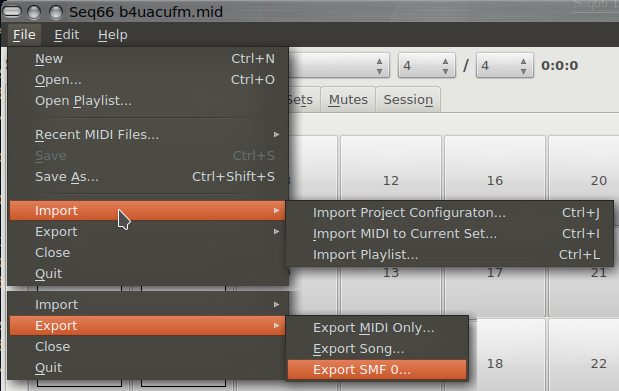
\includegraphics[scale=0.75]{main-menu/file/livegrid-dark-menu-file-2.png}
   \caption{Seq66 Menu File Items, Composite View}
   \label{fig:menu_file_items}
\end{figure}

   \begin{enumber}
      \item \textbf{New}
      \item \textbf{Open}
      \item \textbf{Open Playlist}
      \item \textbf{Recent MIDI files}
      \item \textbf{Save}
      \item \textbf{Save As}
      \item \textbf{Import}
      \begin{enumber}
         \item \textbf{Import Project Configuration...}
         \item \textbf{Import MIDI to Current Set...}
         \item \textbf{Import Playlist...}
         \index{restart!automatic}
         Once the playlist is imported,
         \textsl{Seq66} is automatically \textsl{\textbf{restarted}}
         in order to load the playlist.
         Be careful!
      \end{enumber}
      \item \textbf{Export}
      \begin{enumber}
         \item \textbf{Export MIDI Only...}
         \item \textbf{Export Song...}
         \item \textbf{Export SMF 0...}
      \end{enumber}
      \item \textbf{Quit} (\textbf{Exit} in \textsl{Windows})
   \end{enumber}

   For information on the \textbf{File} menu when \textsl{Seq66} is
   running under the \textsl{Non Session Manager}, see
   \sectionref{subsubsec:sessions_file_menu}.

\subsection{Menu / File / New}
\label{subsec:menu_file_new}

   The \textbf{New} menu entry clears the current song.
   (A play-list or mute-groups setup, if loaded, are not affected.)
   If unsaved changes are pending, the user is prompted to save the changes.
   Prompting for changes is more comprehensive than \textsl{Seq24}.
   However, when in doubt, save!
   Keep backups of your tunes and configuration files!

\subsubsection{Menu / File / Open}
\label{subsubsec:menu_file_open}

   The \textbf{Open} menu entry opens a song (MIDI file or \textsl{Cakewalk}
   WRK file), replacing the current song (after a prompt if the song was
   modified).
   It opens up a standard file dialog:

\begin{figure}[H]
   \centering 
   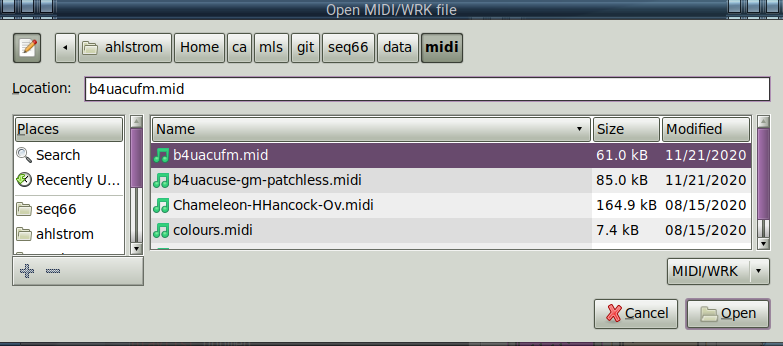
\includegraphics[scale=0.65]{main-menu/file/light-menu-file-open.png}
   \caption{File / Open}
   \label{fig:menu_file_open}
\end{figure}

   This dialog lets one type a file-name, highlighting the first file
   that matches the characters typed.
   \textsl{Seq66} can open \textsl{Seq66}, MIDI SMF 0, and SMF 1 files, and
   \textsl{Cakewalk} WRK files.
   If the file is an SMF 0 file, where all channels appear on one track, the
   track is split so that each channel (0 to 15) is stored in the corresponding
   pattern, and pattern 16 contains the original track.

\subsubsection{Menu / File / Open Playlist}
\label{subsubsec:menu_file_open_playlist}

   The \textbf{Open Playlist...} menu entry opens a \textsl{Seq66}
   play-list file.

\begin{figure}[H]
   \centering 
   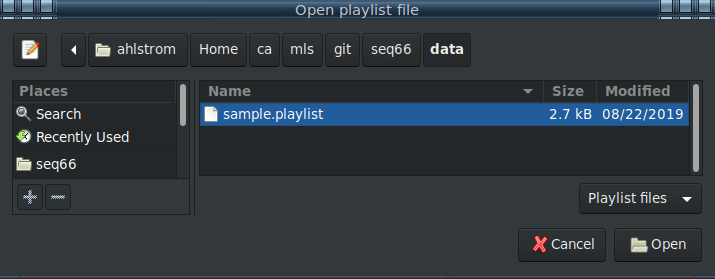
\includegraphics[scale=0.65]{main-menu/file/dark-menu-file-open-playlist.png}
   \caption{File / Open Playlist}
   \label{fig:menu_file_open_playlist}
\end{figure}

   The playlist file contains a list of "playlist sections",
   each listing a number of MIDI songs.
   These playlists and songs can be
   selected by the arrow keys or by MIDI control,
   and are displaed and editiable in the \textsl{Playlist} tab
   in the main window.
   See \sectionref{sec:playlist}.

\subsubsection{Menu / File / Recent MIDI files}
\label{subsubsec:menu_file_recent}

   This menu entry provides a list of the last few MIDI files created or opened;
   play-list selections are \textsl{not} included in this list.

\begin{figure}[H]
   \centering 
   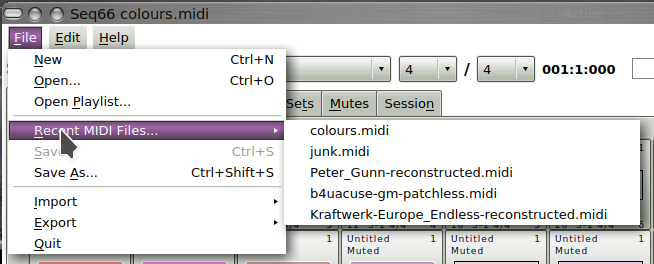
\includegraphics[scale=0.65]{main-menu/file/menu-recent-files.png}
   \caption{Seq66 Menu File Recent Files}
   \label{fig:menu_file_recent_files}
\end{figure}

   Here is the long form when the 'rc' file's
   \texttt{[recent-files] full-paths} value is set to true:

\begin{figure}[H]
   \centering 
   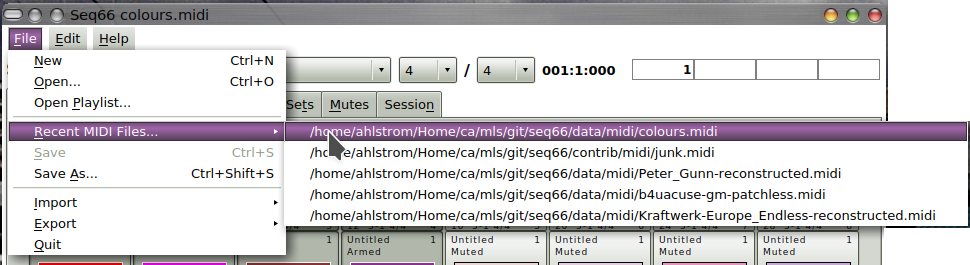
\includegraphics[scale=0.65]{main-menu/file/menu-recent-files-long.png}
   \caption{Seq66 Menu File Recent Files, Full Paths}
   \label{fig:menu_file_recent_files_full_paths}
\end{figure}

   This list is saved in the \texttt{[recent-files]} section of the
   'rc' configuration file.
   In the 'rc' file, the full path to the file-name is stored.
   This path is in "UNIX" format, using the forward slash, or solidus,
   as the path separator, even in \textsl{Windows}.
   The \texttt{full-paths} option can be set to show the full path in the
   recent-files drop-down menu.
   Only unique entries are included in the recent-files list.
   The limit is 12 recent-file entries.
   This is a feature from \textsl{Kepler34} \cite{kepler34}.
   One can also set \textsl{Seq66} to load the most-recent file at startup.
   Here is an example from an 'rc' file:

\begin{verbatim}
   [recent-files]
   full-paths = false
   load-most-recent = true
   count = 3
   /home/user/git/seq66/data/b4uacuse-gm-patchless.midi
   /home/user/git/seq66/data/midi/colours.midi
   /home/user/git/Julian-data/TestBeeps.midi
\end{verbatim}

\subsubsection{Menu / File / Save and Save As}
\label{subsubsec:menu_file_open_save_as}

   The \textbf{Save} menu entry saves the song under its current file-name.
   If there is no current file-name, it opens up a standard file
   dialog to name and save the file.
   The \textbf{Save As} menu entry saves a song under a different name.
   It opens up the following standard file dialog, very similar to the 
   \textbf{File Open} dialog, with an additional \textbf{Name} text-edit field.

\begin{figure}[H]
   \centering 
   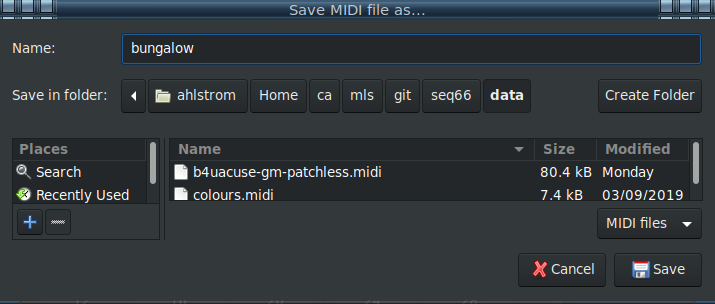
\includegraphics[scale=0.65]{main-menu/file/dark-menu-file-save-as.png}
   \caption{File / Save As}
   \label{fig:menu_file_save_as}
\end{figure}

   To save a new file or save the current file to a new name,
   enter the name in the name field, without an extension.
   \textsl{Seq66} will append a \texttt{.midi} extension to the filename.
   The file will be saved in a format that the Linux \textsl{file} command
   will tag as something like:

   \begin{verbatim}
      colours.midi: Standard MIDI data (format 1) using 16 tracks at 1/192
   \end{verbatim}

   It looks like a simple MIDI file, and yet, if one re-opens it in
   \textsl{Seq66}, one sees that the mute-groups, labeling, pattern
   information, and song layout have been preserved in this file.
   This information is saved in a way that MIDI-compliant software
   should be able to use or ignore without failure.
   After the last track in the file, a number of
   \index{SeqSpec}
   sequencer-specific (SeqSpec) items are saved, to preserve
   the extra information that \textsl{Seq66} adds to the song.
   There is no way to save a \textsl{Cakewalk} "WRK" file.
   \textsl{Seq66} can only read them, and then save them as
   \textsl{Seq66} files.

   \index{Meta events}
   Meta events are now partially handled by \textsl{Seq66}.
   Meta events \textbf{Set Tempo}
   and \textbf{Time Signature}
   are now fully supported.
   Other meta events,
   such as \textbf{Meta MIDI Channel}
   and \textbf{Meta MIDI Port}
   are now read as events, and are saved back when the file is saved.
   They cannot be edited in \textsl{Seq66}, but they are not lost.
   (Channel and port meta events are
   considered \textsl{obsolete} in the MIDI standard.)

\subsubsection{Menu / File / Import / Import Project Configuration}
\label{subsubsec:menu_file_import_project_configuration}

   This command is useful to grab an existing project configuration
   (i.e. the set of \texttt{qseq66.*} files) and copy it
   to another directory.
   This command is most useful in importing a project into a new
   NSM session.  Previously, the "home" project would be imported automatically
   into a new NSM session, but this was deemed confusing by some users, and
   properly so!

   This command brings up a file dialog box. Navigate to the desired
   source directory and then select the desired 'rc' file.

   If importing into an NSM session, one must use the NSM user-interface
   (\textsl{agordejo}, \textsl{RaySession}, or \textsl{nsm-legacy-gui}
   to \textsl{Stop} and then \textsl{Start} \textsl{Seq66}.
   This saves and rereads the configuration.
   If importing into a normal (i.e. not NSM) session, \textsl{Seq66} will
   restart itself automatically to save and reread the configuration.
   Be aware!

   Also note that importing a playlist is a separate operation (see
   below).

\subsubsection{Menu / File / Import / Import MIDI to Current Set}
\label{subsubsec:menu_file_import}

   The \textbf{Import} menu entry imports an SMF 0
   or SMF 1 MIDI file as one or more patterns, one pattern per track,
   into the specified screen-set.
   This functionality is explained in detail in
   \sectionref{subsubsec:midi_export_file_import}.

\subsubsection{Menu / File / Import / Import Playlist}
\label{subsubsec:menu_file_import_playlisMIDI to Current Sett}

   A user can create a playlist that accesses MIDI files anywhere in the file
   system.
   However, in a session manager, it is preferable to have the configuration
   self-contained.
   Even without a session manager, it can be useful to copy a playlist to a
   subdirectory in order to separate it and its MIDI files from other
   playlists.
   Once a project has been imported or saved, then a playlist can also be
   imported, along with all of the MIDI files it references.

   This command brings up a file dialog box. Navigate to the desired
   source directory and then select the desired 'playlist' file.
   This menu entry does a lot of things; here are the steps it performs:

   \begin{itemize}
      \item Copies the selected playlist file into the current configuration
         directory.  This directory is one of the following:
         \begin{itemize}
            \item The default "home" directory,
               \texttt{\textasciitilde/.config/seq66}.
            \item A "home" directory specified by the \texttt{--home} option.
            \item The session directory created by \textsl{NSM}.
         \end{itemize}
         For discussion, this directory is called "HOME".
      \item In HOME, creates a directory called \texttt{playlist/listname},
         where "listname" is the base part of the playlist name, as in
         \texttt{listname.playlist}.
      \item The playlist is opened, parsed, and all of the MIDI tunes specified
         in that file are copied into the new playlist directory, preserving
         the directory directory structure of the original playlist.
      \item The 'rc' file is modified to specify the new playlist,
         specify that it is \texttt{active},
         to specify the new \texttt{base-directory} for all of the tunes,
         and to specify that the playlist will be saved at exit.
      \item Lastly, if not running within NSM, \textsl{Seq66} will be
         \index{restart!automatic}
         \textsl{\textbf{restarted}} automatically to load the new,
         active playlist.
         Within NSM, the user must stop and restart \textsl{Seq66}
         manually in the NSM user-interface..
   \end{itemize}

\subsubsection{Menu / File / Export / Export Song as MIDI}
\label{subsubsec:menu_file_export}

   Thanks to the \textsl{Seq32} project, the ability to export songs to MIDI
   format has been added.  In this export, a complete song performance is
   recoded so that other MIDI sequencers can play the performance properly.
   This functionality is explained in detail in
   \sectionref{subsubsec:midi_export_song_export}.

\subsubsection{Menu / File / Export / Export MIDI Only}
\label{subsubsec:menu_file_export_midi_only}

   Sometimes it might be useful to export only the non-vendor-specific
   (non-SeqSpec) data from a \textsl{Seq66} song, in order to reduce the
   size of the file or to accomodate non-compliant sequencers.
   This functionality is explained in detail in
   \sectionref{subsubsec:midi_export_file_export_midi_only}.

\subsubsection{Menu / File / Export / Export SMF 0}
\label{subsubsec:menu_file_export_smf_0}

   This feature is new since version 0.97.  It allows all tracks in the song to
   be consolidated and exported in MIDI's SMF 0 format.  It follows the same
   rules as song export.
   See \sectionref{subsubsec:midi_export_file_export_smf_0}.

\subsection{Menu / Edit}
\label{subsec:menu_edit}

   The \textbf{Edit} menu has undergone some expansion in \textsl{Seq66}.

   \begin{enumber}
      \item \textbf{Preferences...}
      \item \textbf{Song Editor}
      \item \textbf{Apply Song Transpose}
      \item \textbf{Clear Mute Groups}
      \item \textbf{Reload Mute Groups}
      \item \textbf{Mute All Tracks}
      \item \textbf{Unute All Tracks}
      \item \textbf{Toggle All Tracks}
      \item \textbf{Copy Current Set}
      \item \textbf{Paste To Current Set}
   \end{enumber}

   \setcounter{ItemCounter}{0}      % Reset the ItemCounter for this list.

   \itempar{Preferences}{edit!preferences}
   This entry brings up a \textbf{Preferences} menu entry,
   to allow viewing and tweaking MIDI I/O ports, displays options, JACK
   options, and more.
   It can also be brought up by \texttt{Ctrl-P}.
   It is discussed in detail in a later section.

   \itempar{Song Editor}{edit!song editor}
   \index{song editor}
   This item toggles the presence of the main song / performance editor.
   Note that the song editor is also available in the
   \textbf{Song} center tab in the main window.
   The song editor allows specifying exact numbers of loop replays;
   this provides a canned rendition of the MIDI tune.

   \itempar{Apply Song Transpose}{edit!song transpose}
   \index{song transpose}
   Selecting this item applies the global song transposition value to
   all sequences / patterns marked as transposable.
   This actively changes the note / pitch value of all note and aftertouch
   events in the pattern.
   Normally, drum tracks are \textsl{not} transposable.
   For the setting of global song transpose, see
   \sectionref{sec:song_editor}.
   Note that transpose can be enabled in the
   in the sequence editor
   (see \sectionref{sec:pattern_editor}).

   \itempar{Clear Mute Groups}{edit!clear mute groups}
   \index{mute groups}
   A feature of \textsl{Seq66} is that the mute groups
   are saved in both the 'rc' file \textsl{and} in the "MIDI" file.
   This menu entry clears them. If this resulted in any mute-group sequences
   status being set to false, then the user is prompted to save the MIDI
   file, so that it will no longer have any
   mute-group information.  And then, if the
   application exits, the cleared mute-group information is also saved to
   the 'rc' file.

   \itempar{Reload Mute Groups}{edit!load mute groups}
   \index{rc!mute groups}
   This menu entry reloads the mute-groups from the 'rc' file.
   So, if one loads a MIDI file that has its own mute groups that one does not
   like, this command will restore one's favorite mute-grouping from the 'rc'
   file.

   \itempar{Mute All Tracks}{edit!mute all tracks}
   \index{mute all}
   This menu entry, useful mostly in \textbf{Live} mode,
   immediately mutes \textsl{all} patterns in the entire song.
   The hard-wired keyboard short-cut for this action is \texttt{Ctrl-M}.

   \itempar{Unmute All Tracks}{edit!unmute all tracks}
   \index{unmute all}
   This menu entry, useful mostly in \textbf{Live} mode,
   immediately unmutes \textsl{all} patterns in the entire song.
   The hard-wired keyboard short-cut for this action is \texttt{Ctrl-U}.

   \itempar{Toggle All Tracks}{edit!toggle all}
   \index{toggle all}
   This option toggles the mute/armed status of \textbf{all} tracks.
   It is useful mostly \textbf{Live} mode, which overrides \textbf{Song}
   mode even if the Song Editor is focussed.
   The hard-wired keyboard short-cut for this action is \texttt{Ctrl-T}.

   \itempar{Copy Current Set}{edit!copy set}
   \index{copy set}
   This item marks the current set for the copying of all its patterns to
   another set.
   After clicking this menu entry, one can move to another set to paste it,
   using the following menu entry.

   \itempar{Paste To Current Set}{edit!paste set}
   \index{paste set}
   If a set has been marked for the copying of all its patterns to
   another set, then this menu item is enabled.
   Move to the desired set (whether empty or note), and then
   click this menu item.
   All of the patterns in the original set are pasted into the current set.

\subsubsection{Menu / Edit / Preferences}
\label{subsubsec:menu_edit_preferences}

   \textbf{Preferences} provides a number of settings in one
   tabbed dialog, shown in the figures that follow.
   It allows one to set MIDI clocking, MIDI Input, display tweaks, minor
   playback options, and some JACK parameters.

  Configuration items not (yet) implemented in \textbf{Preferences} are
      incoming MIDI events to control the sequencer;
      what keys are mapped to functions;
      how the mouse works, and a few other.
   The MIDI and Key controls, far more numerous than in \textsl{Seq24}, have
   been consolidated into a 'ctrl' file and are fairly easy to edit with a text
   editor.
   \textsl{Seq66} does not support the 'fruity' mouse mode at this time.

\paragraph{Menu / Edit / Preferences / MIDI Clock}
\label{paragraph:menu_edit_preferences_midi_clock}

   The \textbf{MIDI Clock} tab provides a way to set MIDI clocking for
   the available MIDI output busses.
   It configures the output busses for MIDI clock and data.
   It shows the devices that can play music.
   The items that appear in this tab depend on:

   \begin{itemize}
      \item What MIDI devices are connected to the computer.
         MIDI controllers, USB MIDI cables, applications with virtual
         ports, and other connected devices will add MIDI
         output devices (ports) to the system.
         This list will generally match the output of \texttt{aplaymidi -l}
         or \texttt{aconnect -lio}.
      \item The setting of the "manual-ports" option, which tells
         \textsl{Seq66} to set up virtual MIDI ports.
         It is enabled by the
         \texttt{-{}-manual-ports} command-line option or the
         \texttt{[manual-ports]} section of the
         \texttt{qseq66.rc} configuration file,
         or in the \textbf{MIDI Input} tab described below.
      \item The setting of the \textsl{Seq66}-specific
         "reveal ALSA ports" option,
         \texttt{-{}-reveal-ports} command-line option or the
         \texttt{[reveal-ports]} section of the
         \texttt{qseq66.rc} configuration file.
   \end{itemize}

   If \texttt{-{}-manual-ports} is on, this list shows the virtual
   MIDI output busses that \textsl{Seq66} can drive.
   One needs to use a JACK or ALSA MIDI
   connection application to connect a device on each of those outputs.
   The fact that the the buss names can
   start with different numbers, depending on the system setup, can complicate
   the playing of MIDI in this manner.  Also, the 'usr' configuration file can
   change the visible names of the ports to match specific equipment attached
   to the ports.

\begin{figure}[H]
   \centering 
   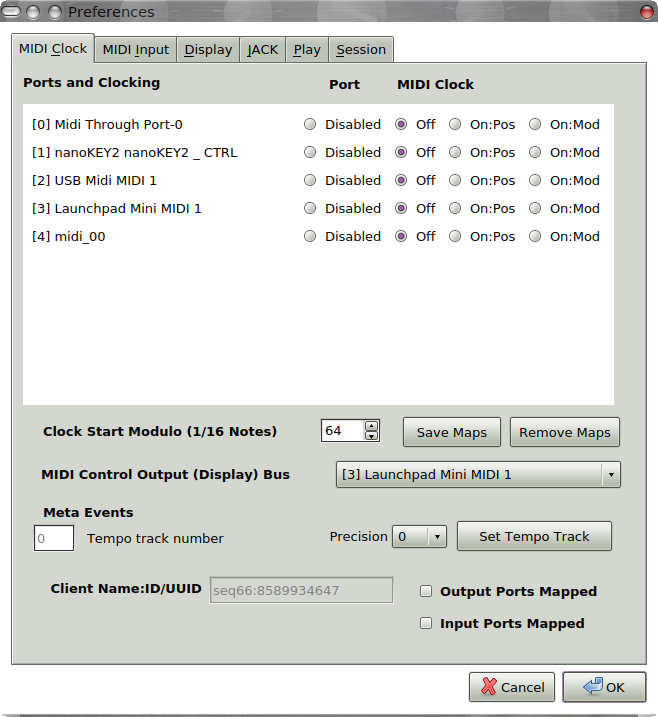
\includegraphics[scale=0.75]{main-menu/edit/preferences/midi_clock_tab.png}
   \caption{MIDI Clock Tab}
   \label{fig:midi_clock_tab}
\end{figure}

   The following elements are present in this tab:

   \begin{enumber}
      \item \textbf{Ports and Clocks Table}
      \item \textbf{Clock Start Modulo}
      \item \textbf{Save Maps}
      \item \textbf{Remove Maps}
      \item \textbf{MIDI Control Output Bus}
      \item \textbf{Meta Events}
      \item \textbf{Client Name:ID/UUID}
      \item \textbf{Output Ports Mapped}
      \item \textbf{Input Ports Mapped}
   \end{enumber}

   \setcounter{ItemCounter}{0}      % Reset the ItemCounter for this list.

   \itempar{Ports and Clocks}{output!ports and clocks}
   \index{output ports}

   This table shows the available MIDI outputs and their status.
   If the set of system MIDI devices and software devices has changed since
   the last run, this list could be in error.  Restart the application
   and see if it is now correct.  Currently, there is no way to edit the list
   except in the 'rc' file.  Also, enabling port-mapping is an issue.

   The \textbf{Ports and Clocks} table contains the following elements,
   although some can be removed by specifying the
   \texttt{port-naming = short} option in the 'rc' file.

   \begin{enumber}
      \item \textbf{Index Number}
      \item \textbf{Client Number}
      \item \textbf{Port Number}
      \item \textbf{Buss Name}
      \item \textbf{Port Disabled}
      \item \textbf{Off}
      \item \textbf{On (Pos)}
      \item \textbf{On (Mod)}
      \item \textbf{Clock Start Modulo}
   \end{enumber}

   The format of the left side of the entry listing is like the following
   when the port-naming option is "long", and the
   MIDI subsystem is ALSA):

   \begin{verbatim}
      [5] 128:4 yoshimi:input
       ^  ^   ^ ^        ^
       |  |   | |        |
       |  |   | |         ---- Port/buss name
       |  |   |  ------------- Client name
       |  |    --------------- Port/buss number
       |   ------------------- Client number
        ---------------------- Index number
   \end{verbatim}

   \setcounter{ItemCounter}{0}      % Reset the ItemCounter for this list.

   \itempar{Index Number}{midi clock!index number}
   \index{index number}
   The number in square brackets is an ordinal indicating the position
   of the output buss in the list.
   For all practical purposes in \textsl{Seq66}, it \textsl{is} the
   buss/port number.  This number can be stored in a pattern in order to have
   the pattern's output go to that buss.  
   This is true even if port-mapping is in place.
   \index{port!mapping}
   \index{buss!mapping}
   \index{port!override}
   \index{buss!override}
   It can be used with the \texttt{-b},
   \texttt{-{}-buss}, or \texttt{ -{}-bus} options to redirect all
   pattern output to that buss, useful if only one buss is active or the
   \textsl{Seq66} patterns route to non-existent busses.
   (See \sectionref{subsubsec:introduction_sets_buss_override},
   and \sectionref{subsubsec:usr_file_user_midi_settings}.)

   \itempar{Client Number}{midi clock!client number}
   \index{client number}
   The number that precedes the colon is the "client number".
   It is useful mainly in ALSA, where clients can have numbers like "14",
   "128", "129", etc.  For native JACK mode, it matches the index number or is
   the name of the client (e.g. "seq66").

   \itempar{Port Number}{midi clock!port number}
   \index{port number}
   The number that follows the colon is the "port number".
   It is useful mainly in ALSA.
   For native JACK mode, it matches the index number.

   \itempar{Buss Name}{midi clock!buss name}
   \index{port name}
   \index{midi clock!port name}
   These labels indicate the output busses (ports) available.
   \textsl{Seq66} does not access devices by name, but by port number.
   However, a port-map can be created to make it possible to find the correct
   buss / port number by name lookup.

   \itempar{Port Disabled}{midi clock!port disabled}
   The \textbf{Port Disabled} clock choice marks an output port
   that the user does not want to use or that the operating system
   (\textsl{Windows} \smiley)
   is locking or disabling.
   Normally, this inaccessible port would cause \textsl{Seq66} to exit.
   With the port disabled, the inaccessible port is ignored.
   This feature also shows when a port-map cannot find a device in the system's
   device list.
   When the \textsl{Windows} version of \textsl{Seq66}
   (\texttt{qpseq66.exe}) is first started, it may error out.
   It will then write a default \texttt{qseq66.rc}
   or \texttt{qpseq66.rc} configuration file,
   which can be examined to find the offending buss, which can then be
   marked in the normal 'rc' file as disabled.

   \itempar{Off}{midi clock!off}
   Disables the MIDI \textsl{clock} for the given output buss.
   MIDI output is still sent to those ports, and
   each port that has a device connected to it will play music.
   Some synthesizers may require this setting.

   \itempar{On (Pos)}{midi clock!on (pos)}
   MIDI clock will be sent to this buss.
   MIDI Song Position and MIDI Continue will be sent if playback starts
   at greater than tick 0 in Song mode.  Otherwise, MIDI Start will be sent.
   Note: In case of trouble, see
   \sectionref{subsec:alsa_testing}.

   \itempar{On (Mod)}{midi clock!on (mod)}
   MIDI clock will be sent to this buss.
   MIDI Start will be sent, and clocking will begin
   once the Song Position has reached the start modulo of the specified size
   (see the next item's description).
   This setting is used for gear that does not respond to Song Position.

   Below the \textbf{Ports and Clocks Table} are more configuration elements.

   \setcounter{ItemCounter}{0}      % Reset the ItemCounter for this list.

   \itempar{Clock Start Modulo}{midi clock!clock start modulo}
   Clock Start Modulo (1/16 Notes).
   This value starts at 1 and ranges up to 16384, and defaults to 64.
   It is used by the \textbf{On (Mod)} setting discussed above.
   It is the \texttt{[midi-clock-mod-ticks]} option in the \textsl{Seq66}
   'rc' file.

   \itempar{Save Maps}{midi i/o!port mapping}
   \index{port mapping}
   \index{port!mapping}
   Pressing this button saves the current set of MIDI I/O ports to sections in
   the 'rc' file.  These sections can be enabled in order to support
   port-mapping in subsequent runs of \textsl{Seq66}.
   Generally, after pressing this option, one will want to stop
   \textsl{Seq66}, rearrange the clock and input maps in the
   'rc' file with a text editor, back up this file in a safe place,
   and restart \textsl{Seq66}.

   \itempar{Remove Maps}{midi i/o!remove mapping}
   \index{remove mapping}
   \index{port! remove mapping}
   Pressing this button removes the port mapping.
   \index{restart!manual}
   Once done, either restart \textsl{Seq66} or go to the \textbf{Session}
   tab and click the \textbf{Reload Session} button.
   (See \sectionref{subsec:concepts_reload_session}.)

   \itempar{MIDI Control Output Bus}{midi control!output buss}
   \index{midi control!output}
   Use this control to select the output bus used to display
   application-automation status, loop status, and mute-group status.
   Requires a \textsl{reload session} to take effect.
   The number of the buss is stored in the 'ctrl' file named in
   \sectionref{paragraph:menu_edit_preferences_session},
   as the value of \texttt{output-buss}.
   If port mapping is enabled (now the default),
   the nick-name of the bus is stored instead of the number.

   \itempar{Meta Events}{midi clock!meta events}
   \index{tempo-track-number}
   This section consists of the following items:

   \begin{enumerate}
      \item \textbf{Tempo track number}
      \item \textbf{Precision}
   \end{enumerate}

   \textbf{Tempo track number}
   allows the user to move the tempo track from pattern 0 to
   another pattern.  Changing this option is not recommended, since track 1 (0)
   is the official track for tempo events, but \textsl{Seq66} allows the
   user to record tempo events to another track.  \textsl{Seq66} will
   process tempo events in any pattern.
   \textsl{The "Set as Tempo Track" button to the right is not yet functional.}

   \index{usr!bpm-precision}
   \textbf{Precision}
   allows setting the number of digits past the decimal point to 0, 1, or 2.
   This is also a 'usr' setting.
   See \sectionref{subsubsec:usr_file_user_midi_settings}.
   The BPM (tempo) is stored in the MIDI file multiplied by 1000 to accommodate
   the decimal places.

   \itempar{Client Name:ID/UUID}{client ID}
   This read-only text field shows two things:

   \begin{enumerate}
      \item \textbf{Client Name}.
         This is the name of the client under ALSA or JACK.  It defaults to
         \texttt{seq66}, but it can be altered by the command-line option
         \texttt{-{}-client-name} or by a session manager.
         Each instance of Seq66 run under ALSA will have a different client ID.
      \item \textbf{ID/UUID}.
         Under ALSA, the client number (client ID) is shown.
         Under JACK, the UUID that JACK assigned to \textsl{Seq66} is shown.
   \end{enumerate}

   \itempar{Output Ports Mapped}{mapping!output}
   This check-box shows if the port-mapper is active for the output ports.
   It becomes set if the \textbf{Save Maps} button is clicked, and unset if the
   \textbf{Remove Maps} button is clicked.
   Uncheck this button and \textsl{reload session} for the setting
   to take effect.

   \itempar{Input Ports Mapped}{mapping!input}
   This check-box shows if the port-mapper is active for the input ports.
   It becomes set if the \textbf{Save Maps} button is clicked, and unset if the
   \textbf{Remove Maps} button is clicked.
   Uncheck this button and \textsl{reload session} for the setting
   to take effect.

%  \index{todo!manual alsa gui option}
%  There is currently no user-interface item corresponding to the "manual-ports"
%  command-line and 'rc' configuration file option.
%  We should rename this option to "virtual" eventually.

\paragraph{Menu / Edit / Preferences / MIDI Input}
\label{paragraph:menu_edit_preferences_midi_input}

   To set up \textsl{Seq66} to record MIDI from devices such as
   controllers and keyboards, the output of the ALSA MIDI recording
   command-line \texttt{arecordmidi -l} is relevant.
   Something like that listing appears in the Input tab:

\begin{figure}[H]
   \centering 
   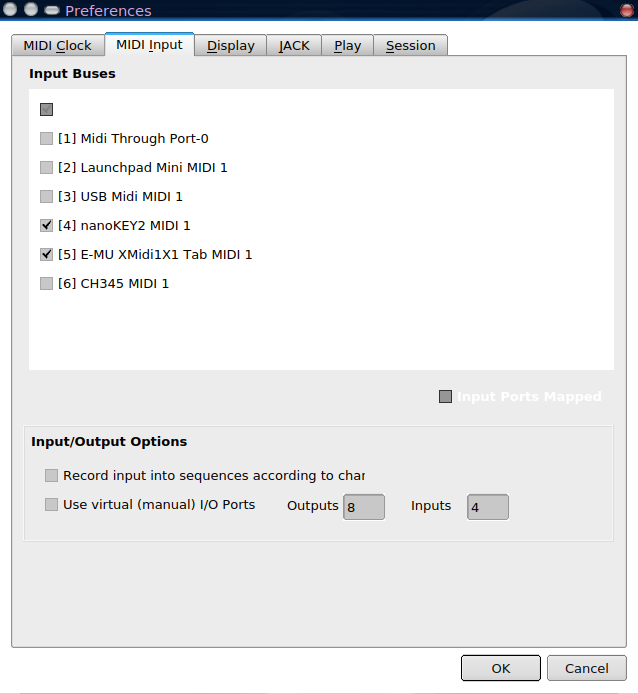
\includegraphics[scale=0.75]{main-menu/edit/preferences/midi_input_tab.png}
   \caption{MIDI Input, ALSA View}
   \label{fig:midi_input_tab}
\end{figure}

   Any item checked allows \textsl{Seq66} to record MIDI from that source,
   which must be connected to this input port.

   \textbf{Warning:}
   \index{warnings!usr config}
   \index{usr config}
   If the 
   \texttt{[user-midi-bus-definitions]} value in the 'usr' configuration file
   is non-zero, and the
   corresponding number of
   \texttt{[user-midi-bus-N]} settings are provided, then
   the list of existing hardware will be ignored, and those values will be
   shown instead.
   This feature can be overridden with the
   \texttt{-{}-reveal-ports} (\texttt{-r}) option.
   If you define these sections, they should match your
   hardware exactly, and your hardware should not change from session to
   session.
   If the "auto ALSA ports" option is turned on, via the \texttt{-a} or
   \texttt{-{}-auto-ports} option, then
   the input ports from the system are shown.

   \setcounter{ItemCounter}{0}      % Reset the ItemCounter for this list.

   \itempar{Input Buses}{input buses}
   \textbf{Input Buses} delineates the MIDI input devices as noted above.

   \itempar{MIDI Control Input Bus}{midi control!input buss}
   \index{midi control!input}
   Use this control to select the input bus used for MIDI control automation of 
   application actions, loop actions, and mute-group actions.
   Requires a \textsl{reload session} to take effect.
   The number of the buss is stored in the 'ctrl' file named in
   \sectionref{paragraph:menu_edit_preferences_session},
   as the value of \texttt{control-buss}.
   If port mapping is enabled (now the default),
   the nick-name of the bus is stored instead of the number.

   \itempar{Input Options}{input options}
   \index{input options}
   \textbf{Input Options} adds further refinements to MIDI input.
   Currenty it has only one setting, for recording input into patterns by the
   channel in each event.

   \itempar{Input/Output Recording}{record!by channel}
   \index{input by channel}
   \textbf{Record input into sequence according to channel}
   causes MIDI input with multiple channels to be distributed to
   each sequence according to MIDI channel number.
   When disabled, the normal recording behavior dumps all data into the current
   sequence, regardless of channel.

   \itempar{Input/Output Virtual Ports}{ports!virtual}
   \textbf{Use virtual (manual) I/O Ports}
   This new option
   allows for configuration of the manual-ports option from within the
   user-interace. 
   Once the option is enable
   A \textsl{reload session} (see \sectionref{subsec:concepts_reload_session})
   is necessary for this option to take effect.

\paragraph{Menu / Edit / Preferences / Keyboard}
\label{paragraph:menu_edit_preferences_keyboard}

   Unlike \textsl{Seq24}, \textsl{Seq66}
   \textsl{does not} provide an options tab for
   setting up the keyboard.
   The default keyboard mappings follow \textsl{Seq24} fairly well,
   but add a large number of additional controls;
   around 96 keystroke slots would need to be provided!
   The keystroke and MIDI controls are consolidated, and are easy to change by
   editing the appropriate 'ctrl' configuration file, stored in one of the
   following directories, depending on
   the operating system:
   
   \begin{verbatim}
         /home/username/.config/seq66/qseq66.ctrl           (Linux)
         C:/Users/username/AppData/Local/seq66/qpseq66.ctrl (Windows)
   \end{verbatim}

   There are also some extended examples present in the \textsl{Seq66}
   \texttt{data/linux} and
   \texttt{data/samples} directory.
   Also see \sectionref{sec:launchpad_mini}.
   For more information on keystrokes, see
   \sectionref{subsec:kbd_mouse_keyboard_control}.

\paragraph{Menu / Edit / Preferences / Mouse}
\label{paragraph:menu_edit_preferences_mouse}

   Unlike \textsl{Seq24}, \textsl{Seq66}
   \textsl{does not} provide an options tab for
   the mouse-interaction method.
   It is not supported in \textsl{Seq66}...
   the "Fruity" interaction method is not available;
   only the "Seq24" interaction is available.
 
\paragraph{Menu / Edit / Preferences / Display}
\label{paragraph:menu_edit_preferences_display}

   This dialog provides a few odds and ends to enhance the user-interface.
   Some of these items (plus a few more) can be configured by editing the 'usr'
   file.

\begin{figure}[H]
   \centering 
   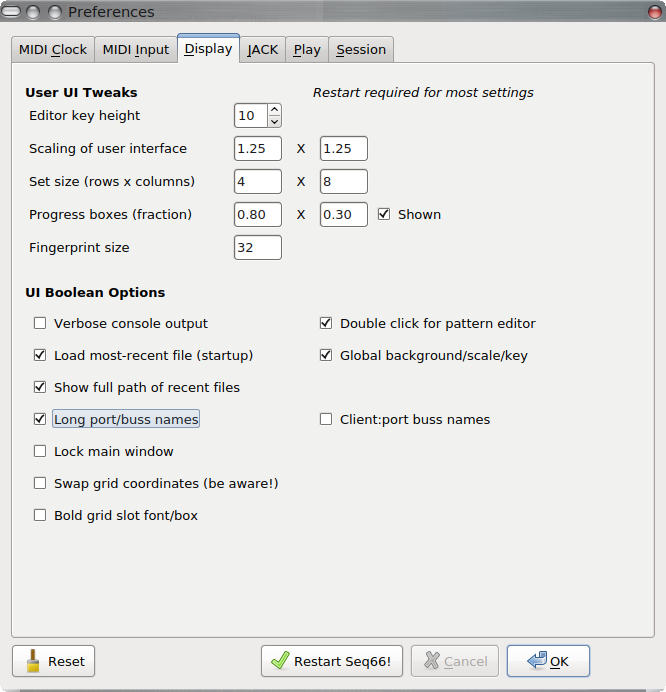
\includegraphics[scale=0.75]{main-menu/edit/preferences/midi_display_tab.png}
   \caption{Display Options}
   \label{fig:midi_display_tab}
\end{figure}

   \setcounter{ItemCounter}{0}      % Reset the ItemCounter for this list.

   \itempar{Editor Key Height}{key height}
   This option affects the pattern editor's piano roll.  Smaller means a wider
   range of notes can be shown.  There are also
   \textbf{-},
   \textbf{0}, and
   \textbf{+} buttons in the pattern editor that provide
   vertical zoom.

   \itempar{Scaling of User Interface}{window scaling}
   These two items set scale factor for width and height of the main window.
   The lowest scale factor is 0.5, and the largest scale factor is 3.0.
   For the smallest window, the smallest practical values are 0.85 x 0.60.

   \itempar{Set Size}{set-size}
   Provides a way to change the set size.  The default is
   \textbf{4 x 8}
   (rows by columns), but we intend to support
   \textbf{4 x 4},
   \textbf{8 x 8}, and
   \textbf{12 x 8}
   as well.

   \textbf{Warning}:
   A different set size alter the 'ctrl' file radically.
   We still have to work through all the implications of changing the set size,
   so back up your configuration and proceed with caution!

   \itempar{Progress Boxes}{progress-box size}
   Provides a way to change the size of the progress box in each button.
   Values are width and height fractions (up to 1.0) re the button size.
   This is a 'usr' option.

   \itempar{Progress Box Shown}{progress-box shown}
   If the \textbf{Shown} check-box
   is \textsl{unchecked}, then the progress boxes and pattern color are not
   shown.
   This is a 'usr' option.

   \itempar{Fingerprint Size}{fingerprint size}
   This value, if set from 32 to 128, indicates the number of events above
   which a "fingerprint", rather than every note, will be drawn.  It can
   save some CPU time in drawing the grid.  If set to 0, the whole
   pattern is drawn, no matter how long the pattern is.

   \itempar{Verbose Console Output}{verbose}
   This boolean makes more output appear if \textsl{Seq66} is run from a
   console/terminal. It will also increase the amount of data logged to the log
   file, if activated.

   \itempar{Load Most Recent File (startup)}{load most-recent}
   If checked, the file at the top of the \texttt{[recent-files]}
   list in the 'rc' file is loaded at startup.

   \itempar{Show Full Path of Recent Files in Menu}{full paths}
   The full path of each file in the \texttt{[recent-files]} list
   is shown in the menu.  Although they can be uncomfortably long, they can
   show files that have the same name, but in different directores.

   \itempar{Long Port/Buss Name}{buss names!long}
   \index{buss names!short}
   Controls how much port information is shown in the clocks and input
   listings.  For the "portmidi" (e.g. \textsl{Windows})
   implementation, keep this option checked.

   \itempar{Lock Main Window}{main window!lock}
   This item makes the window non-resizable after startup.

   \itempar{Swap Coordinates}{grid!swap coordinates}
   Normally, \textsl{Seq66} displays the pattern and mute-groups grids
   where the pattern numbers increase fastest downward.
   Some might prefer to have pattern numbers increase fastest rightward.
   This setting make the patterns show in the more conventional manner.

   \textbf{Warning}:

      \begin{itemize}
         \item This setting requires the 'ctrl' file to be rewritten
            if one want to preserve the normal layout for the pattern hot-keys
            and the mute-group hot-keys.
         \item This setting has not been rigorously tested, so be prepared for
            some issues.
      \end{itemize}

   A 'ctrl' file for the swapped setting is provided
   in \texttt{qseq66-swapped.ctrl} in the \texttt{data/linux}
   directory, but it might not be completely correct yet.

   \itempar{Bold Slot Font}{grid!bold}
   \index{font!bold}
   \index{progress bar!thick}
   This setting makes the font in the live grid bold, and it allows
   make the progress-bar thick in the grid and in the Live and Song piano
   rolls.
   It is the same as the \texttt{progress-bar-thick = true} option in the 'usr'
   file. See \sectionref{subsubsec:usr_file_user_interface_settings}.

   \itempar{Double click for pattern editor}{grid!bold}
   \index{double-click!pattern slot}
   If set, a double-click on a grid button brings up the pattern for editing.
   Disable it if the effect is confusing.

   \itempar{Global background/scale/key}{globals!background etc.}
   \index{global pattern setting!background}
   \index{global pattern setting!key}
   \index{global pattern setting!scale}
   If set, setting the background sequence, scale to show, or the key of the
   track will apply to all pattern windows that are opened.

   \itempar{Client:port buss names}{buss!naming}
   \index{bus!naming}
   If checked the MIDI engine's "client:port" numbers are shown in the port
   listings.
 
\paragraph{Menu / Edit / Preferences / JACK}
\label{paragraph:menu_edit_preferences_jack}

   This tab sets up JACK transport, if \textsl{Seq66}
   was built with JACK support (\textsl{Linux} only).

\begin{figure}[H]
   \centering 
   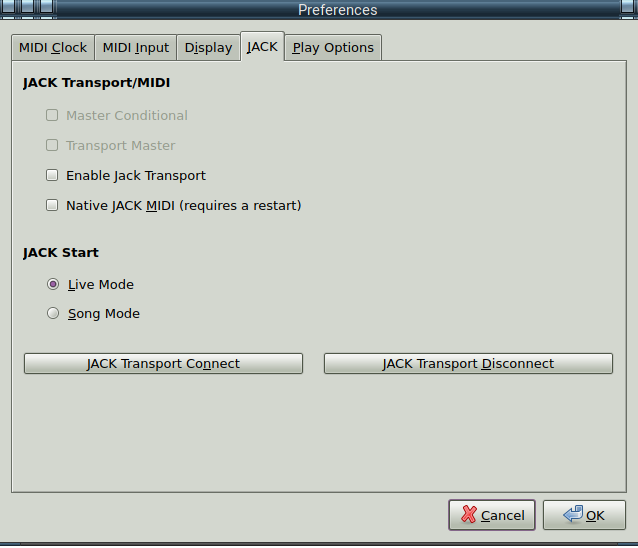
\includegraphics[scale=0.75]{main-menu/edit/preferences/midi_jack_tab.png}
   \caption{Edit / Preferences / JACK}
   \label{fig:midi_jack_tab}
\end{figure}

   The main sections in this dialog are:

   \begin{enumber}
      \item \textbf{JACK Transport/MIDI}
      \item \textbf{JACK Start Mode}
      \item \textbf{JACK Transport Connect and Disconnect}
   \end{enumber}

   \setcounter{ItemCounter}{0}      % Reset the ItemCounter for this list.

   \itempar{Transport/MIDI}{jack sync!transport/midi}
   These settings are stored in the 'rc' file settings group
   \texttt{[jack-transport]}.
   This items collects the following settings:

   \begin{itemize}
      \item \textbf{Jack Transport}.
         \index{JACK!transport}
         Enables slave synchronization with JACK Transport.
         The command-line option is \texttt{-{}-jack-transport}.
         The behavior of this mode of operation is perhaps not quite
         correct.  Even as a slave, \textsl{Seq66} can start and
         stop playback.
         Note that this option cannot be disabled via the mouse if the
         \textbf{Transport Master} option is enabled.  Disable that one first.
      \item \textbf{Transport Master}.
         \index{JACK!transport master}
         \textsl{Seq66} will attempt to serve as the JACK Master.
         The command-line option is \texttt{-{}-jack-master}.
         \textbf{Tip}:
         \textsl{Seq66} generally works better as JACK Master.
         If this option is enabled the \textbf{JACK Transport} option is
         automatically enabled as well.
      \item \textbf{Master Conditional}.
         \index{JACK!master conditional}
         \textsl{Seq66} will fail to serve as the JACK Master if there is
         already a Master.
         The command-line option is \texttt{-{}-jack-master-cond}.
         If this option is enabled the \textbf{JACK Transport} option is
         automatically enabled as well.
      \item \textbf{Native JACK MIDI}.
         \index{JACK!native midi}
         This option is for the \texttt{qseq66} (Linux) version of
         \textsl{Seq66}.
         If set, MIDI input and output use native JACK MIDI,
         rather than ALSA.  However, if JACK is not running on the
         system, then \texttt{seq66} will fall back to ALSA mode.
         (However, if \texttt{jackdbus} is running, but the JACK engine is not,
         then a couple of non-working manual ports are created.  To be fixed in
         the future.)
         The command-line option is \texttt{-{}-jack-midi}
         or \texttt{-{}-jack}.
      \item \textbf{JACK Auto-Connect}.
         \index{JACK!auto-connect}
         This option has been true for a long time in \textsl{Seq66}, and
         non-configurable.  Now it can be turned off, in order to let the user
         or a session manager make the connections, even when not using
         manual/virtual ports.
   \end{itemize}

   If one makes a change in the JACK transport settings, it is best to
   then press the \textbf{JACK Transport Disconnect} button, then the
   \textbf{JACK Transport Connect} button.
   Another option is to restart
   \textsl{Seq66}... the settings are automatically saved when
   \textsl{Seq66} exits.

   \itempar{JACK Start mode}{jack sync!start mode}
   This item collects the following settings, also stored in the 'rc' file
   settings group \texttt{[jack-transport]}.

   \begin{itemize}
      \item \textbf{Live Mode}.
         \index{JACK!live mode}
         \index{live mode}
         \index{non-playback mode}
         Playback will be in live mode.  Use this option to allow muting and
         unmuting of patterns.  This option might also be called "non-song
         mode".
         The command-line option is \texttt{-{}-jack-start-mode 0}.
      \item \textbf{Song Mode}.
         \index{JACK!song mode}
         \index{song mode}
         \index{playback mode}
         \index{performance mode}
         Playback will use only the Song Editor's data.
         The command-line option is \texttt{-{}-jack-start-mode 1}.
   \end{itemize}

   \textsl{Seq66} also selects the playback modes
   according to which window started the playback.
   \textsl{The main window}, or pattern
   window, causes playback to be in live mode.  The user can arm and mute
   patterns in the main window by clicking on sequences, using their hot-keys,
   and by using the group-mode and learn-mode features.
   The song editor causes playback to be in performance mode, also known as
   "playback mode", or \textbf{Song} mode.

   \itempar{Connect}{jack sync!connect}
   Connect to JACK Sync.
   This button is useful to restart JACK sync when making changes to it,
   or when \textsl{Seq66} was started in ALSA mode.

   \itempar{Disconnect}{jack sync!disconnect}
   Disconnect from JACK Sync.
   This button is useful to stop JACK sync when making changes to it.
   JACK connection and disconnection are disabled during playback, but the
   buttons don't yet reflect that status.

\paragraph{Menu / Edit / Preferences / Play Options}
\label{paragraph:menu_edit_preferences_play_options}

   This tab contains some disparate options ostensibly related to playback.

\begin{figure}[H]
   \centering 
   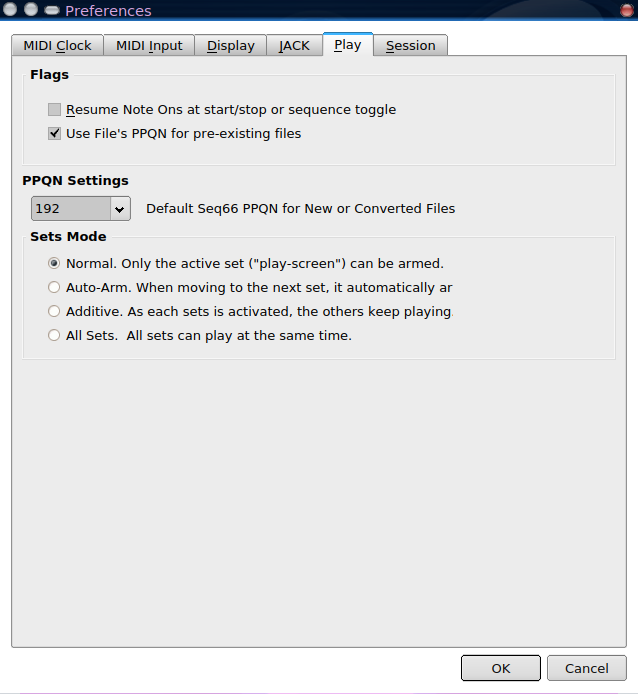
\includegraphics[scale=0.75]{main-menu/edit/preferences/midi_play_options_tab.png}
   \caption{Play Options}
   \label{fig:midi_play_options_tab}
\end{figure}

   \setcounter{ItemCounter}{0}      % Reset the ItemCounter for this list.

   \itempar{Resume Note Ons...}{edit!resume notes}
   \textbf{Resume Note Ons at start/stop or sequence toggle}
   allows notes that had already started
   to be resumed when playback resumes.

   \itempar{Use File's PPQN...}{edit!use file ppqn}
   \textbf{Use File's PPQN for Pre-Existing Files}, if checked, allows
   \textsl{Seq66} to run using the PPQn of the MIDI file rather than
   the default \textsl{Seq66} internal PPQN.
   When this option is changed, the \texttt{-{}-user-save} option is turned on
   to preserve the setting when \textsl{Seq66} exits.

   \itempar{Default Seq66 PPQN...}{edit!default ppqn}
   \textbf{Default Seq66 PPQN for New or Converted Files}, if checked, allows
   the standard PPQN, 192 pulses/quarter-note, to be changed to discrete values
   from 32 to 19200.  Intermediate values, even oddball values, can be entered
   by typing the number directly.
   When this option is changed, the \texttt{-{}-user-save} option is turned on
   to preserve the setting when \textsl{Seq66} exits.
   If there is a MIDI file loaded, it is modified to use the new PPQN, and the
   user is prompted to save it at exit.

   \itempar{Sets Mode}{edit!sets-mode}
   This item determines how sets are handled.
   Recall that a set is a number of patterns (up to 4x8) in the pattern grid,
   and that the current set is the one visible in the pattern grid.
   The way sets work in \textsl{Seq66} is that, when a set is selected,
   all the patterns in it are loaded into what is called
   the "play-set".
   When play starts only, patterns in the play-set are handled.
   The \textbf{Sets Mode} option allows special handling of the play-set.

   \begin{enumerate}
      \item \textbf{Normal}.
         In this mode, only the current set's patterns can be unmuted.
         When switching to another set, the current set's patterns become
         muted, and the new set's patterns are shown, unmuted.
      \item \textbf{Auto-Arm}.
         Here, when the new set is loaded, it is immediately unmuted.
      \item \textbf{Additive}.
         With this option, when a new set is loaded, the previous set keeps
         playing. This allows a build-up of patterns in playback.
      \item \textbf{All Sets}.
         Here, all sets in the tune are loaded and unmuted at once.
         Try this mode with the \texttt{b4uacuse-stress.midi} file
         in the \textsl{Sequencer64} project.  It's a good test of
         \textsl{Seq66} and your hardware/software synthesizer!
   \end{enumerate}

   One can clear the out play-set, and set only the current set active, by
   clicking the exclamation point button to the left of the "Active" label at
   the bottom of the main windows.

\paragraph{Menu / Edit / Preferences / Metronome Options}
\label{paragraph:menu_edit_preferences_metronom_options}

   This tab contains options for the "metronome" and
   "background recording" features:

\begin{figure}[H]
   \centering 
   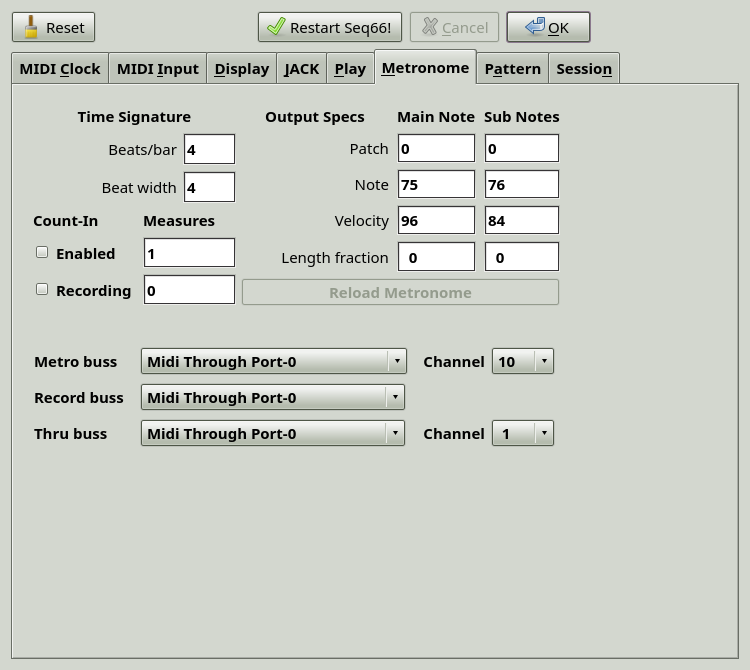
\includegraphics[scale=0.80]{main-menu/edit/preferences/midi_metro_options_tab.png}
   \caption{Metronome Options}
   \label{fig:midi_metro_options_tab}
\end{figure}

   \setcounter{ItemCounter}{0}      % Reset the ItemCounter for this list.

   The metronome feature is enabled in the main live grid via a metronome
   button.
   The metronome is a standard \textsl{Seq66} pattern, but it is never seen
   nor edited by the user.
   It is not saved with a song, so changing the metronome does not modify the
   song.
   The settings shown above are saved to a "metronome" section in the 'rc'
   file.
   The metronome is a pattern that first plays a main note once, and then
   plays "sub" notes for the rest of the measure.
   Here are the settings:

   \itempar{Beats/bar}{metronome!beats/bar}
   This setting sets the beats-per-measure for the metronome only.
   It currently does not affect the time-bar in the main window.
   Should it? There is a global beats/bar as well as beats/bar for
   each pattern.

   \itempar{Beat width}{metronome!beat width}
   This setting sets the beat width for the metronome only.
   The following settings are provided for the "main" note
   (the note that occurs on the beginning of the measure)
   and the "sub" notes (the notes that occur on each beat):

   \itempar{Patch}{metronome!patch}
   This item sets the program (patch) number for the note, which sets the
   instrument to play for the notes.
   We currently do not have a drop-down box to select the patch by name.
   The default patch is 0.
   As noted below, the default channel is 10, so this
   patch is the "Standard Drum Kit" for the device.
   Thus, by default the metronome can be implemented by two different
   drums.

   \itempar{Note}{metronome!note}
   This item provides the note value to be played.  Recall that 60 is the same
   as "middle C".  By default, the main note is 75, the "Clave" for the drum
   kit, and the sub note is 76, the "High Wood Block" for the drum kit.

   \itempar{Velocity}{metronome!velocity}
   This item provides the note velocity to be played, to provide an accent on
   the main note.

   \itempar{Length Fraction}{metronome!length fraction}
   The length of the notes are specified as a fraction of the beat width, and
   this value ranges from 0.125 to 1.0 to 2.0.
   If set to 0, the length is half of the beat width.

   \itempar{Reload Metronome}{metronome!reload}
   This button pauses playback (if playing),
   loads in the new metronome settings, and
   continues playing (if it was playing).
   It is \textsl{not} enabled when the status/configuration of background
   recording changes.

   \itempar{Metro Buss}{metronome!buss}
   This value selects the output MIDI device to use to play the metronome.
   It \textsl{must} be enabled in the \textbf{MIDI Clock} list.

   \itempar{Channel}{metronome!channel}
   This value selects the channel to use to play the metronome.

   \itempar{Record Buss}{recorder!buss}
   \index{background recorder}
   This value selects the input device to use to record events into the
   background pattern.
   Note that this device \textsl{must be enabled} in the \textbf{MIDI Input}
   buss list.

   \itempar{Thru Buss}{record!thru buss}
   This value selects the output MIDI device to use to play the incoming
   background record notes.  Otherwise they will not be heard.
   It \textsl{must} be enabled in the \textbf{MIDI Clock} list.

   \itempar{Thru Channel}{recorder!thru channel}
   This value selects the channel to use to play the recorded notes as
   they come in.

   We still have some more work to do to refine the metronome, the
   background recorder, and their configuration, pending user input.

\paragraph{Menu / Edit / Preferences / Session}
\label{paragraph:menu_edit_preferences_session}

   This tab contains options related to session management and the
   configuration files.

\begin{figure}[H]
   \centering 
   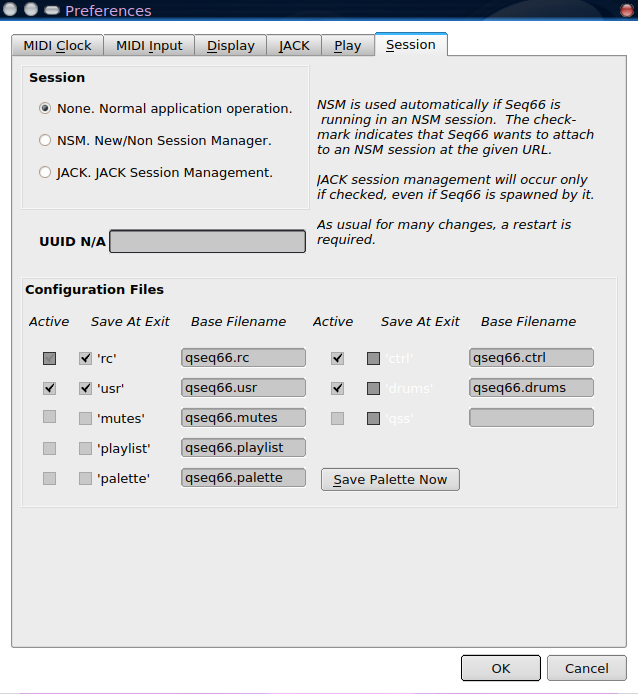
\includegraphics[scale=0.75]{main-menu/edit/preferences/midi_session_tab.png}
   \caption{Session Options}
   \label{fig:midi_session_options_tab}
\end{figure}

   \setcounter{ItemCounter}{0}      % Reset the ItemCounter for this list.

   \itempar{Session}{edit!session}
   \textbf{Session}
   This section provides for three modes of session management:  None, the
   Non/New Session Manager (NSM), and JACK Session management.
   None is the normal mode of operation, where the user has full control of
   where to put files, what other applications are to be run alongside
   \textsl{Seq66}, and what connections are to be made.

   NSM provides a rigorously-controlled session management, and directs
   \textsl{Seq66} what menu items to display, whether to hide the
   user-interface or not, where configuration files and MIDI files go, and what
   applications are run in a session. It can also (via \texttt{jackpatch}) keep
   a record of connections to reconstruct.

   JACK Session provides a location for file and a record of applications and
   connections, but otherwise lets the user mess things up.  It is
   provided because some people still use it.
   For more information about session management, see
   \sectionref{sec:sessions}.

   \itempar{UUID}{edit!UUID}
   \textbf{UUID} is a read-only field that shows any UUID that's relevant to a
   session. Normally has a value only in a \textsl{JACK} or
   \textsl{NSM} session.
   Also see the \textbf{Session} tab in the main window
   (\sectionref{sec:sessions}).

   \itempar{Configuration Files}{edit!configuration}
   \textbf{Configuration Files}
   shows the status of the configuration files.
   (See \sectionref{subsec:configuration_rc}).
   The 'rc' file is always active, and normally is saved at exit (even if no
   configuration changes occurred).

   The 'usr' file should also be active, but one can disable it, which is
   currently an \textsl{experimental} and \textsl{untested} option.
   Normally, it is not saved at application exit (except after the first run on
   one's system).
   (See \sectionref{subsec:configuration_usr}).

   The rest of the configuration files are optional.
   See
   \sectionref{subsec:configuration_ctrl},
   \sectionref{subsubsec:configuration_mute_group_control},
   \sectionref{subsec:configuration_drums}, and
   \sectionref{sec:playlist}.

   \itempar{Palette File Base Name}{palette}
   This text edit holds the base name of a 'palette' file, which is always
   stored in the \textsl{Seq66} configuration directory.
   (See \sectionref{sec:palettes}.)

   \itempar{Save Current Palette}{palette}
   Normally, there is no palette file.  Pushing this button creates one, which
   can then be modified and configured as the palette-file to use in the 'rc'
   file.

\subsection{Menu / Help}
\label{subsec:menu_help}

   The usual \textbf{Help} dialog is provided.
   As of version 0.98.8, it has been beefed up with a way to access a
   tutorial and the user manual.

   These new help items are a work in progress, so please apprise
   us of any issues; include information on the operating system and,
   if \textsl{Linux}, the desktop/window manager in use.

\subsubsection{Menu / Help / About...}
\label{subsubsec:menu_help_about}

   \index{Help!about}
   This menu entry shows the "About" dialog.
   That dialog provides access to some credits for the program as well.
   authors and the project documentors, and active link to them.
   It also shows Git version-control information as well.

\subsubsection{Menu / Help / Build Info...}
\label{subsubsec:menu_help_build_info}

   \index{Help!build info}
   This menu entry shows the "Build Info" dialog.  This list of
   build options enabled in the current application is the same list
   that it generated via this command line:

   \begin{verbatim}
      $ seq66 --version
   \end{verbatim}

\subsubsection{Menu / Help / Song Summary File...}
\label{subsubsec:menu_help_song_summary_file}

   \index{Help!song summary}
   This menu entry allows one to write a summary of the song data into a text
   file. It brings up a file dialog which defaults to the name of the
   currently-loaded MIDI file, with the extenstion \texttt{.text} and
   the directory from where the MIDI file was loaded.
   It shows the filename, number of sets and tracks, MIDI format (0 or 1),
   and the PPQN.

   It also shows each sequence: name, channel (128 mean there is no output
   channel), the time signature, buss number (and any mapping), the length in
   pulses, the event and trigger count, transposability, key and scale, and
   color number (if any).
   For each trigger in the pattern, its start, stop, offset, and transposition
   values are shown.
   This file can be helpful for trouble-shooting or solving puzzling effects in
   the tune.

\subsubsection{Menu / Help / Tutorial}
\label{subsubsec:menu_help_tutorial}

   \index{Help!tutorial}
   This entry brings up a short tutorial of \textsl{Seq66} in the default
   browser. This tutorial is meant only to jump-start a new user of
   \textsl{Seq66}, and is a work in progress.
   It does not cover nearly as much as the user manual, so check that out in
   the next section.

   Normally, the tutorial will open a web page.  If it does not, one might need
   to set up a default browser.  On Linux, make sure that there is a "desktop"
   file for the browser, as in
   \texttt{/usr/share/applications/firefox.desktop}.
   If so, then run the following command, and then test it:

   \begin{verbatim}
      $ xdg-settings set default-web-browser firefox.desktop
      $ xdg-open https://ahlstromcj.github.io/docs/seq66/tutorial/index.html 
   \end{verbatim}

   On Windows, this procedure is still \textsl{to be determined}.

   In both systems, one can override the default applications by opening
   the specified 'usr' file (usually \texttt{qseq66.usr} or
   \texttt{qpseq66.usr} and specifying the full path to the desired
   applications (Linux paths shown here):

   \begin{verbatim}
      [user-options]
      log = "/home/user/.config/seq66/seq66.log"
      pdf-viewer = "/usr/bin/zathura"
      browser = "/usr/bin/google-chrome"
   \end{verbatim}

   Also see \sectionref{subsubsec:usr_file_user_options}.

\subsubsection{Menu / Help / User Manual}
\label{subsubsec:menu_help_user_manual}

   \index{Help!user manual}
   This menu entry first tries to locate the user manual on the internet and
   open it in the default browser. If not found, or the network is down,
   then this entry brings up the full \textsl{Seq66} user manual in the default
   PDF viewer.  It currently looks in the possible installation areas and in
   the \textsl{Seq66} source tree to find the PDF.

   On Linux, one can follow the setup procedure in the previous section and
   test it via the following command, which will show the manual in the default
   browser.:

   \begin{verbatim}
      $ xdg-open https://ahlstromcj.github.io/docs/seq66/seq66-user-manual.pdf
   \end{verbatim}

%-------------------------------------------------------------------------------
% vim: ts=3 sw=3 et ft=tex
%-------------------------------------------------------------------------------
